%!TEX root = ../thesis-main.tex
\chapter{Validation}
\label{chap:validation}
The \textbf{Test Driven Development (TDD)} approach was utilized for testing. TDD is a software development approach where tests are written before any production code. This approach was used during the development of the project to ensure the high quality of the code, to detect and resolve quickly the bugs, and to make any changes to the code confidently. In the basic flow of TDD a developer would follow these steps:
\begin{itemize}
	\item Write a test for a specific feature or behavior of the code.
	\item Run the test and see that it fails (since there is no production code yet).
	\item Write the minimum amount of code necessary to make the test pass.
	\item Run the test again and see that it passes.
	\item Refactor the code if necessary, making sure that all tests still pass.
\end{itemize}
This approach is optimal because it encourages developers to think about the desired behavior of the code before writing it, and to focus on writing code that is easy to test.
Tests become a specification of the desired behavior, which is useful for understanding goals and documenting code.
Tests would also dramatically reduce bug identification and resolution.
Finally, it also helps to ensure that the code is well-structured and easy to maintain, since any changes to the code will be accompanied by corresponding changes to the tests\footnote{https://virtuale.unibo.it/pluginfile.php/1147871/mod\_resource/content/0/01-quality.pdf}.\newline

When an issue or a bug is detected, it is critical to take action to prevent it from happening again. One useful method is to write a test that looks for the problem or bug and fails if it arises again. This is referred to as a \textbf{Regression Test}. When a problem was discovered, a new regression test or an additional assertion was added to the test codebase, strengthening the software.

\section{Automated Testing In Kotlin Multiplatform}
\label{sec:automated-testing-in-kotlin-multiplatform}
By default, Kotlin Multiplatform supports running tests on JVM, JS, Android, Linux, Windows, macOS, iOS, watchOS, and even on tvOS simulators. Other Kotlin/Native targets must be manually configured in an appropriate environment, emulator, or test framework before tests can be run. Since the Alchemist Web Renderer project only uses the Java Virtual Machine and JavaScript as its target platforms, it is only required to perform testing on those specific environments.\newline

The best way to test a Kotlin Multiplatform project is to use the \textit{kotlin.test} library, which provides a common testing framework for all the platforms. The main purpose of the library is to avoid the duplication of test code for each platform and to make it easy to test the common code on all platforms. The multiplatform code will be tested on all the targets it will run on, to ensure that the code is working correctly on each specified target.\newline

Kotest\footnote{https://kotest.io/}, a testing framework for the Kotlin programming language, was also used for testing the project. It can be easily integrated in a Kotlin Multiplatform project, making it a versatile choice for testing. One of its key feature is the ability to make tests easy to read and understand, which can be especially useful for developers working on large projects with many test cases. Additionally, Kotest provides a wide range of assertion functions and test runners, allowing developers to write comprehensive, expressive tests with minimal boilerplate code. A detailed explanation on how the code testing process is conducted across all the different platforms follows now:
\begin{itemize}
	\item \textbf{JVM Testing:} It is crucial to note that different JVMs may behave and function differently depending on their version. This can result in issues or bugs that only appear on certain JVMs. By testing on multiple JVMs, developers can ensure that their code is compatible with the chosen set of JVMs. The application of the \textit{Multi-JVM testing Plugin for Gradle}\footnote{https://github.com/DanySK/multi-jvm-test-plugin} is beneficial for this purpose. The plugin automatically configures a Java (or Kotlin, or other plugins applying Java) build to run tests under multiple versions of the JVM. It exposes support to decide on which JVM to compile code, pre-configures the test task to run on the same JVM, and creates useful additional tasks;
	\item \textbf{JS Testing:} Testing code of the JS platform can be achieved by configuring a variety of test runners via the Gradle configuration. The default configuration relies on the Karma test runner, along with other essential dependencies for browser applications. By default, the multiplatform plugin executes browser tests using headless Chrome. It would still be possible to include other browsers to run tests by customizing the build process;
	\item \textbf{Common Testing:} The tests for shared components are run on all the platforms that the code is intended to support, using the techniques already exposed.
\end{itemize}

The CI automatically checks the \textbf{Coverage} state by using CodeCov\footnote{https://about.codecov.io/} every time new code is submitted to the Alchemist repository. For Kotlin Multiplatform projects, the only included sourcesets in the analysis are common and JVM. In fact, CodeDev depends on the coverage reports generated by JaCoCo\footnote{https://www.jacoco.org/jacoco/index.html}.

\section{Front-end Testing}
\label{sec:front-end-testing}
Tests that focus of the Frontend code can be difficult to automate because they frequently entail user interactions with the interface and testing the application's visual features. Sometimes, specialized tools that simulate user interactions are used, but they can be complex to set up and maintain.\newline

Manual testing, on the other hand, entails a human tester physically engaging with the program, testing its features and its functionalities, rating the overall user experience. Manual testing can be time-consuming and prone to human mistake, but it can provide vital insights into the application's usability and functionality.\newline

It is crucial to note that manual testing does not imply that there is no documentation or process; rather, manual testing requires a clear and well-defined methodology that includes test cases, test scripts, and expected results. Furthermore, testing should be performed not only by developers but also by QA testers, or, even better, by a group of users during the user acceptability testing phase.\newline

The application user interface is really poor in terms of content to display by now, as the project is still in the beginning phase of the development. Other aspects have been considered to be much more important, like the automated testing already discussed in \fullref{sec:automated-testing-in-kotlin-multiplatform}.\newline

For the time being, the application has just undergone functional testing. This type of testing focuses on verifying that the application's features and functionality work as expected. This includes testing the application's inputs, outputs, and the interactions with other systems.\newline

Since the UI is still not ready, performing UX testing may not be effective, as the design and layout of the application may change during development. Additionally, testing the usability of a UI that is not fully implemented may not provide an accurate representation of the final user experience. This is because UX testing involves evaluating the design and layout of the application, as well as the navigation and overall usability.

\section{Performance Evaluation}
\label{sec:performance-evaluation}
At the current stage of development, profiling performance may not be a highly useful exercise, as there are numerous aspects of the project that can be improved. It is worth noting that the primary objective of this research was not to achieve optimal performance, which remains a significant challenge in this particular scenario. Therefore, the focus has been primarily on establishing a solid foundation that can facilitate the development of new features with relative ease, while addressing the known performance issues as development progresses.\newline

Along with some considerations, some data is still being presented. The measurements were performed on a single machine, where both the Server and the Client components are located. The machine has limited hardware capabilities, and is characterized by the following specifications:

\begin{itemize}
	\item \textbf{Processor}: Intel(R) Core(TM) i5-2520M CPU @ 2.50GHz
	\item \textbf{RAM}: 8GiB System memory
	\item \textbf{GPU}: 2nd Generation Core Processor Family Integrated Graphics Controller
\end{itemize}

\paragraph{Free variables}
The two free variable in the measurements are:
\begin{enumerate}
	\item the number of nodes $N$ ($N \in \mathbb{N}^{+}$) participating in the system, representing the size of the monitored system;
	\item The utilized approach (Computation on Server or Computation on Server).
\end{enumerate}
\paragraph{Metrics}
The four metrics measured to evaluate the performance of the system are:
\begin{enumerate}
	\item \textbf{rendering time}: the time required by the renderer component to complete its execution, this
	metric is meant to compare the raw performance of the renderer across the available platforms. The execution on the JVM is expected to be faster than the one on the browser;
	\item \textbf{serialization time}: the time required by the Server to serialize the \textit{Environment State} (in the Computation on Client approach) or the rendered image (in the Computation on Server approach). This operation is always accomplished by the Server;
	\item \textbf{deserialization time}: the time required by the Client to deserialize the \textit{Environment State} (in the Computation on Client approach) or the rendered image (in the Computation on Server approach). This operation is always accomplished by the Client;
	\item \textbf{total time}: the time required to complete an entire iteration, which includes all the previous metrics plus the network delay.
\end{enumerate}

Each metric is measured five times, and the presented results are an average of such data.

\paragraph{Final Results}
The results are presented and summarized in \fullref{fig:performace-graphs}.
\begin{center}
	\begin{figure}[htb]
		\centering
		\begin{subfigure}[t]{0.45\textwidth}
			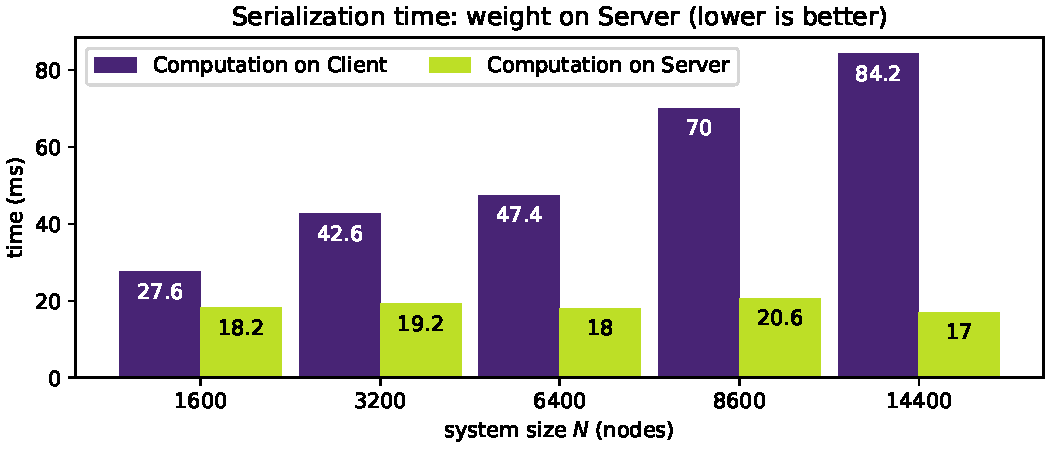
\includegraphics[width=0.99\textwidth]{figures/serialization-time}
		\end{subfigure}%
		~
		\begin{subfigure}[t]{0.45\textwidth}
			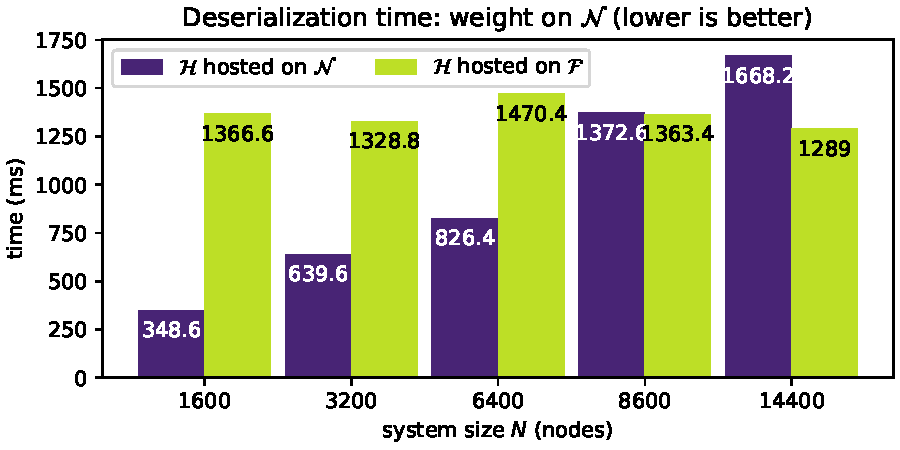
\includegraphics[width=0.99\textwidth]{figures/deserialization-time}
		\end{subfigure}
		~
		\begin{subfigure}[t]{0.45\textwidth}
			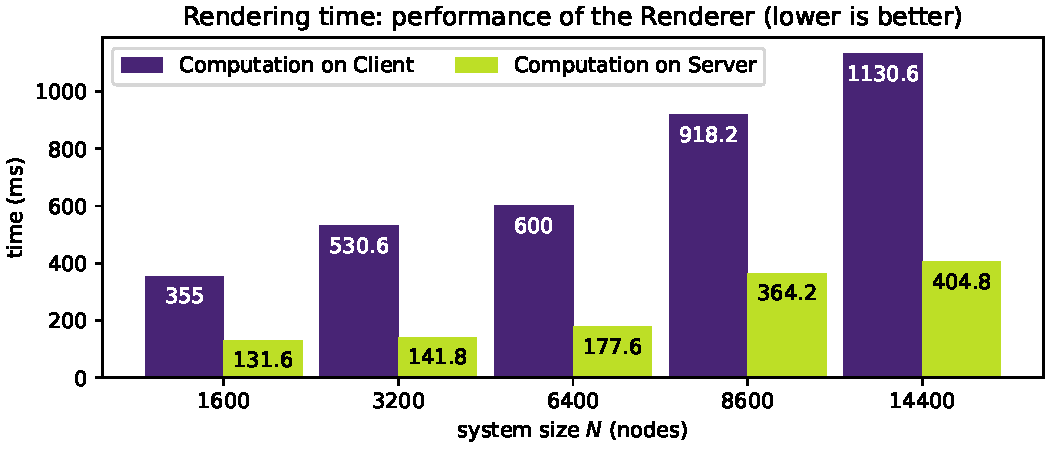
\includegraphics[width=0.99\textwidth]{figures/rendering-time}
		\end{subfigure}
		~
		\begin{subfigure}[t]{0.45\textwidth}
			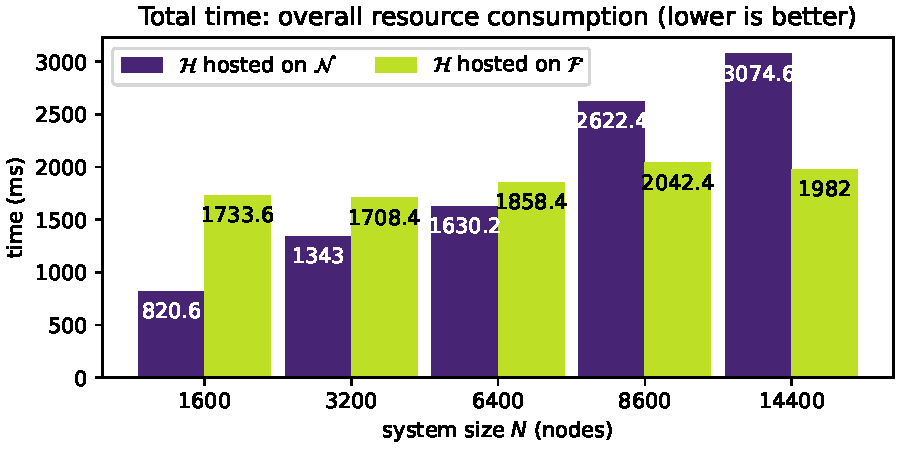
\includegraphics[width=0.99\textwidth]{figures/total-time}
		\end{subfigure}
		\caption{Performance Evaluation - Comparison of the metrics in function of the free variables}
		\label{fig:performace-graphs}
	\end{figure}
\end{center}

As anticipated, utilizing the Computation on Server approach yields more stable system performance as the monitored system expands. This is mainly due to the JVM's superior efficiency in comparison to Javascript. Additionally, the JVM is consistently faster in rendering the system and surprisingly quicker in converting the model into an image format than in plain JSON. Nevertheless, this is highly reliant on the specific serialization formats and libraries employed, and may drastically change with different implementations. Finally, it is apparent that adopting the Computation on Client approach is quite effective for minor systems, but it becomes less scalable than the Computation on Server strategy as the environment size expands.
